
\begin{figure*}
\centering
\subfloat[Figure A][\label{fig:webrtcA}
$p_1$ connects to $p_2$ using the signaling service. 
1: $p_1$ pushes its offer ticket; 
2: $p_2$ pulls the ticket; 
3: $p_2$ pushes its response; 
4: $p_1$: pulls the response and establishes a 
connection with $p_2$. $p_3$ does the same with $p_2$. 
%%Figure~\ref{fig:webrtcB} depicts the resulting network.
]{
  
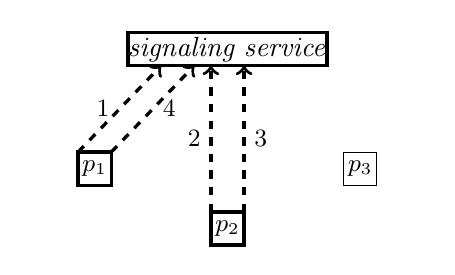
\begin{tikzpicture}[scale=1.2]

\newcommand\X{40pt};
\newcommand\Y{18pt};

\draw( 1.5*\X, 0); %% spacing
\draw(-1.5*\X, 0); %% spacing

\draw[fill=white,very thick](0*\X, 0*\Y) 
node{\emph{signaling service}} +(-30pt,-5pt) rectangle +(30pt,5pt);

\small
\draw[->,dashed, very thick](-5 -1*\X, 5-2*\Y) --
node[anchor=east]{1} (-20pt,-5pt);
\draw[->,dashed, very thick]( 5 -1*\X, 5-2*\Y) --
node[anchor=west]{4} (-10pt,-5pt);

\draw[->,dashed, very thick](-5pt,  5-3*\Y) --
node[anchor=east]{2}(-5pt,-5pt);
\draw[->,dashed, very thick](5pt , 5-3*\Y) --
node[anchor=west]{3} (5pt,-5pt);


\draw[fill=white, very thick]
(-1*\X,-2*\Y) node{$p_1$} +(-5pt,-5pt) rectangle +(5pt,5pt);
\draw[fill=white, very thick]
(0*\X, -3*\Y) node{$p_2$} +(-5pt,-5pt) rectangle +(5pt,5pt);
\draw[fill=white] (1*\X, -2*\Y) node{$p_3$} +(-5pt,-5pt) rectangle +(5pt,5pt);

\end{tikzpicture}

% \begin{tikzpicture}
% \matrix (m) [matrix of math nodes,row sep=4em,column sep=4em] {
% \node(ss)[draw]{signaling}; & \node(p3)[draw]{p3}; \\
% \node(p1)[draw]{p1}; & \node(p2)[draw]{p2}; \\
% };
% \path[->]
%   (p2) edge[dashed] node[fill=white]{1:emit} (ss)
%   (p3) edge[dashed] node[fill=white,bend left]{2:pull} (ss)
%   (p3) edge[dashed, bend right] node[fill=white]{3:accept} (ss)
%   (p2) edge[dashed,bend left] node[fill=white]{4:pull} (ss)
%   (p3) edge[<->,thick] node[fill=white,right]{5:connected} (p2);
% \end{tikzpicture}}
\hspace{5pt}
\subfloat[Figure B][\label{fig:webrtcB}
$p_1$ connects to $p_3$ using $p_2$ as mediator. 
1: $p_1$ sends its offer ticket to $p_2$; 
2: $p_2$ forwards it to $p_3$ and registers $p_1$ as the emitter; 
3: $p_3$ sends its response to $p_2$; 
4: $p_2$ forwards it to the emitter $p_1$ which connects to $p_3$.]{
  
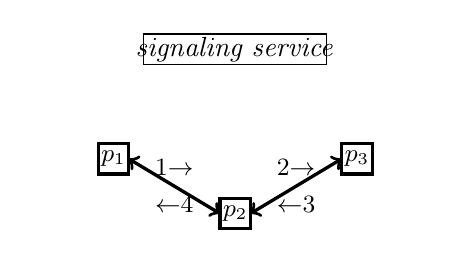
\begin{tikzpicture}[scale=1.1]

\newcommand\X{40pt};
\newcommand\Y{18pt};

\draw(1.7*\X, 0); %% spacing
\draw(-1.7*\X, 0); %% spacing

\draw[fill=white](0*\X, 0*\Y)
node{\emph{signaling service}} +(-30pt,-5pt) rectangle +(30pt,5pt);

\small
\draw[<->, very thick](5-1*\X,-2*\Y)--
node[anchor=south]{1$\rightarrow$}
node[anchor=north]{$\leftarrow$4}(-5pt,-3*\Y);
\draw[<->, very thick](5pt,-3*\Y)--
node[anchor=south]{2$\rightarrow$}
node[anchor=north]{$\leftarrow$3}(-5+1*\X,-2*\Y);

\draw[fill=white, very thick]
(-1*\X,-2*\Y) node{$p_1$} +(-5pt,-5pt) rectangle +(5pt,5pt);
\draw[fill=white, very thick]
(0*\X, -3*\Y) node{$p_2$} +(-5pt,-5pt) rectangle +(5pt,5pt);
\draw[fill=white, very thick]
(1*\X, -2*\Y) node{$p_3$} +(-5pt,-5pt) rectangle +(5pt,5pt);

\end{tikzpicture}

% \begin{tikzpicture}
% \matrix (m) [matrix of math nodes,row sep=4em,column sep=4em] {
% \node(ss)[draw]{signaling}; & \node(p3)[draw]{p3}; \\
% \node(p1)[draw]{p1}; & \node(p2)[draw]{p2}; \\
% };
% \path[->]
%   (p1) edge[dashed,bend left] node[fill=white]{1:emit} (p2)
%   (p2) edge[dashed,bend left] node[fill=white,left]{2:emit/p1} (p3)
%   (p3) edge[dashed,bend left] node[fill=white,right]{3:accept/p1} (p2)
%   (p2) edge[dashed,bend left] node[fill=white]{4:accept} (p1)
%   (p1) edge[<->,thick] (p2)
% %  (p1) edge[<->,thick,bend left] (p3)
%   (p2) edge[<->,thick]  (p3);

% \end{tikzpicture}}
\hspace{5pt}
\subfloat[Figure C][\label{fig:webrtcC}
The resulting network overlay: a fully connected network composed of
3 members.]{
  
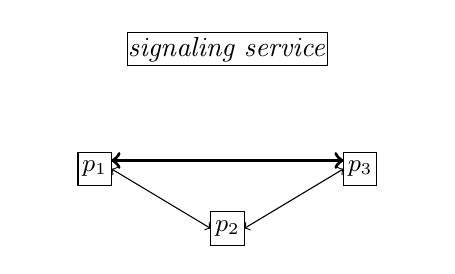
\begin{tikzpicture}[scale=1.2]

\newcommand\X{40pt};
\newcommand\Y{18pt};

\draw(1.5*\X, 0); %% spacing
\draw(-1.5*\X, 0); %% spacing

\draw[fill=white](0*\X, 0*\Y)
node{\emph{signaling service}} +(-30pt,-5pt) rectangle +(30pt,5pt);

\small
\draw[<->](5-1*\X,-2*\Y)--(-5pt,-3*\Y);
\draw[<->](5pt,-3*\Y)--(-5+1*\X,-2*\Y);
\draw[<->, very thick](5 - 1*\X, 2.5 -2*\Y)--(-5+1*\X, 2.5 -2*\Y);

\draw[fill=white]
(-1*\X,-2*\Y) node{$p_1$} +(-5pt,-5pt) rectangle +(5pt,5pt);
\draw[fill=white]
(0*\X, -3*\Y) node{$p_2$} +(-5pt,-5pt) rectangle +(5pt,5pt);
\draw[fill=white]
(1*\X, -2*\Y) node{$p_3$} +(-5pt,-5pt) rectangle +(5pt,5pt);

\end{tikzpicture}


% \begin{tikzpicture}
% \matrix (m) [matrix of math nodes,row sep=4em,column sep=4em] {
% \node(ss)[draw]{signaling}; & \node(p3)[draw]{p3}; \\
% \node(p1)[draw]{p1}; & \node(p2)[draw]{p2}; \\
% };
% \path[->]
%   (p1) edge[<->,thick] (p2)
%   (p1) edge[<->,thick] (p3)
%   (p2) edge[<->,thick]  (p3);
% \end{tikzpicture}}
\caption{\label{fig:webrtc}Creating an overlay network on top of WebRTC.}
\end{figure*}


\section{Related work}
\label{sec:relatedwork}

WebRTC allows real-time peer-to-peer communication between browsers even when
complex network settings such as firewalls, proxies or Net Address Translation
(NAT) are involved. However, WebRTC does not manage addressing nor routing. To
establish a connection, the browsers exchange offers and acknowledgments through
a common mediator, e.g., mails, dedicated signaling services~\cite{peerjs},
existing WebRTC connections~\cite{p} etc. Figure~\ref{fig:webrtcA} describes the
very first connection of one peer $p_1$ with another
$p_2$. Figure~\ref{fig:webrtcB} shows that $p_3$ is able to use $p_2$ as
mediator instead of the signaling service. Figure~\ref{fig:webrtcC} shows the
resulting network. Notice that if $p_2$ crashes during the forwarding process,
the connection establishment will fail, even if an alternative route exists as
WebRTC does not manage routing.

% In Figure~\ref{fig:webrtcA}, $p_1$
% wants to connect to $p_2$. Therefore, $p_1$ pushes an offer ticket to a shared
% signaling service. It is worth noting that many signaling services can
% exist. Peer $p_2$ pulls the offer, stamps it and pushes it back to the signaling
% service. Finally, $p_1$ pulls the stamped ticket and establishes a bidirectional
% connection with $p_2$.  Identically, $p_3$ establishes a connection to $p_2$. We
% refer to the round-trip procedure as \emph{three-way handshake}. At this point,
% Peer $p_1$ is able to establish a connection to $p_3$ without the mediation of
% the former signaling service.  Instead, it uses $p_2$ as temporary signaling
% service.  As shown in Figure~\ref{fig:webrtcB}, Peer $p_1$ pushes an offer
% ticket to $p_2$. As $p_2$ is already connected to $p_3$, it forwards the offer
% to $p_3$ and registers $p_1$ as the emitter. Peer $p_3$ stamps the ticket and
% sends it back to $p_2$ who then forwards it back to $p_1$. Upon receipt, $p_1$
% establishes a bidirectional connection with $p_3$.  Notice that if $p_2$ crashes
% during the forwarding process, the connection establishment will fail, even if
% an alternative route exists as WebRTC does not manage routing.

Using signaling services and existing WebRTC connections allows easy
deployment of random peer sampling protocols~\cite{jelasity2004peer} in
browsers that can run on mobile phones or tablets connected to mobile
networks. In this context, it is crucial to keep the number of connections as
low as possible in order to reduce traffic usage and limit resource
consumption.

Random peer sampling protocols~\cite{jelasity2004peer, jelasity2007gossip}
provide each peer with a partial view $\mathcal{P}$ of the network membership
$\mathcal{N}$. They populate the partial views with references to peers chosen
at random among $\mathcal{N}$ following a uniform distribution using local
knowledge only. Their goal is to converge to an overlay network exposing
properties similar to those of random graphs~\cite{erdos1959random}. They
efficiently provide connectedness, robustness, information dissemination etc. A
wide variety of gossip-based protocols use random peer sampling at their
core. For instance, topology optimization protocols~\cite{voulgaris2005epidemic,
  jelasity2009tman} aiming to improve criterion about localization, latency,
preferences etc.

The representatives of random peer sampling protocols using a fixed-size partial
view are Lpbcast~\cite{eugster2003lightweight},
HyParView\cite{leitao2007hyparview} Newscast~\cite{tolgyeski2009adaptive}, and
\CYCLON~\cite{voulgaris2005cyclon}. They have to know \emph{a priori} the
maximum network size to set their parameters accordingly. These decisions cannot
be safely retracted afterwards.

This inflexibility makes it possible to maintains 7 connections in the browser
despite requiring only 4, while, in the following moment, it still maintains 7
connections while 10 would be needed.  \CYCLON's partial views are commonly
oversized compared to the actual network size to prevent having too few
connections per peer, which, consequently, introduces overhead.  When WebRTC is
involved, we need a dynamic peer sampling service that is able to adapt to the
dynamic number of participants.

Network size estimators can introduce adaptiveness in peer sampling. These
approaches either use
\begin{inparaenum}[(i)]
\item sampling techniques~\cite{ganesh2007peer} which analyze a network subset
  and deduce the network size using probabilistic functions,
\item sketching techniques~\cite{baquero2012extrema}
  which use hashing to compress the high amount of data and deduce the network
  size using the collisions,
\item averaging techniques~\cite{jelasity2004epidemic}
  which use aggregations that converge over exchanges to a value which depends
  on the network size.
\end{inparaenum}
Unfortunately, while they can be accurate in their estimation, they imply a
communication overhead and may have strong assumptions (e.g. random graph
topology). However, adaptiveness should introduce a minimum overhead to peer
sampling in WebRTC applications.

\begin{figure*}
  \centering
  \subfloat[Figure A][$p_1$ contacts $p_2$ to join the network. $p_1$ adds
  $p_2$ to its neighborhood. $p_1$ sends its request to $p_2$.]{
    
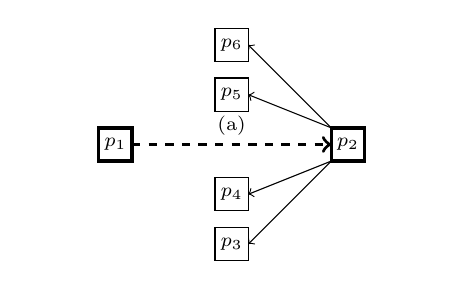
\begin{tikzpicture}[scale=1.2]

  \newcommand\X{35pt};
  \newcommand\Y{15pt};

  \draw(-0.75*\X, 0pt); %% positioning
  \draw( 2.75*\X, 0pt); %% positioning

  \scriptsize
  \draw[->,dashed,very thick](5+0*\X, 0*\Y) -- 
  node[anchor=south]{(a)}(-5+ 2*\X, 0*\Y);
  \draw[->] (-5+2*\X, 5pt) -- (5+\X, \Y);
  \draw[->] (-5+2*\X, 5pt) --  (5+\X, 2*\Y);
  \draw[->] (-5+2*\X, -5pt) -- (5+\X, -\Y);
  \draw[->] (-5+2*\X, -5pt) -- (5+\X, -2*\Y);

  \draw[fill=white, very thick]
  (0*\X, 0*\Y) node{$p_1$} +(-5pt,-5pt) rectangle +(5pt,5pt);
  \draw[fill=white, very thick]
  (2*\X, 0*\Y) node{$p_2$} +(-5pt,-5pt) rectangle +(5pt,5pt);

  \draw[fill=white](1*\X,2*\Y) node{$p_6$} +(-5pt,-5pt) rectangle +(5pt,5pt);
  \draw[fill=white](1*\X,1*\Y) node{$p_5$} +(-5pt,-5pt) rectangle +(5pt,5pt);
  \draw[fill=white](1*\X,-1*\Y) node{$p_4$} +(-5pt,-5pt) rectangle +(5pt,5pt);
  \draw[fill=white](1*\X,-2*\Y) node{$p_3$} +(-5pt,-5pt) rectangle +(5pt,5pt);
  
\end{tikzpicture}}
  \hspace{8pt}
  \subfloat[Figure B][The $onSubs(p_1)$ event is raised at $p_1$
  which forwards the subscription to $p_1$'s neighborhood.]{
    
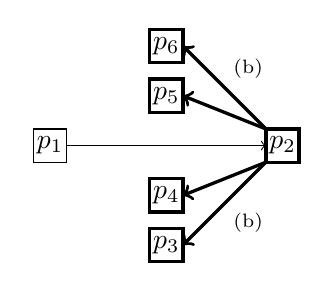
\begin{tikzpicture}[scale=1.2]

  \newcommand\X{35pt};
  \newcommand\Y{15pt};

  \scriptsize
  \draw[->](5+0*\X, 0*\Y) -- (-5+ 2*\X, 0*\Y);
  \draw[->, very thick] (-5+2*\X, 5pt) -- (5+\X, \Y);
  \draw[->, very thick] (-5+2*\X, 5pt) --
  node[anchor=south west]{(b)} (5+\X, 2*\Y);
  \draw[->, very thick] (-5+2*\X, -5pt) -- (5+\X, -\Y);
  \draw[->, very thick] (-5+2*\X, -5pt) --
  node[anchor=north west]{(b)}(5+\X, -2*\Y);

  \normalsize
  \draw[fill=white]
  (0*\X, 0*\Y) node{$p_1$} +(-5pt,-5pt) rectangle +(5pt,5pt);
  \draw[fill=white, very thick]
  (2*\X, 0*\Y) node{$p_2$} +(-5pt,-5pt) rectangle +(5pt,5pt);

  \draw[fill=white, very thick]
  (1*\X,2*\Y) node{$p_6$} +(-5pt,-5pt) rectangle +(5pt,5pt);
  \draw[fill=white, very thick]
  (1*\X,1*\Y) node{$p_5$} +(-5pt,-5pt) rectangle +(5pt,5pt);
  \draw[fill=white, very thick]
  (1*\X,-1*\Y) node{$p_4$} +(-5pt,-5pt) rectangle +(5pt,5pt);
  \draw[fill=white, very thick]
  (1*\X,-2*\Y) node{$p_3$} +(-5pt,-5pt) rectangle +(5pt,5pt);

\end{tikzpicture}}
  \hspace{8pt}
  \subfloat[Figure C][The $onFwdSubs(p_1)$ event is raised at $p_{3-6}$. The 
  peers add $p_1$ to their neighborhood.]{
    
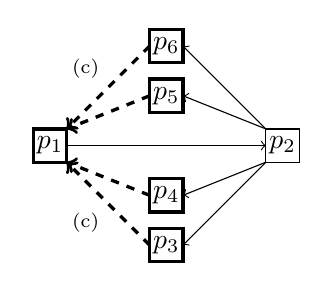
\begin{tikzpicture}[scale=1.2]

  \newcommand\X{35pt};
  \newcommand\Y{15pt};

  \scriptsize
  \draw[->](5+0*\X, 0*\Y) -- (-5+ 2*\X, 0*\Y);
  \draw[->] (-5+2*\X, 5pt) -- (5+\X, \Y);
  \draw[->] (-5+2*\X, 5pt) -- (5+\X, 2*\Y);
  \draw[->] (-5+2*\X, -5pt) -- (5+\X, -\Y);
  \draw[->] (-5+2*\X, -5pt) -- (5+\X, -2*\Y);

  \draw[->,dashed, very thick](-5+\X, 2*\Y) --
  node[anchor=south east]{(c)} ( 5pt,5pt);
  \draw[->,dashed, very thick](-5+\X, 1*\Y) -- ( 5pt,5pt);
  \draw[->,dashed, very thick](-5+\X, -1*\Y) -- ( 5pt,-5pt);
  \draw[->,dashed, very thick](-5+\X, -2*\Y) --
  node[anchor=north east]{(c)}( 5pt,-5pt);

  \normalsize
  \draw[fill=white, very thick]
  (0*\X, 0*\Y) node{$p_1$} +(-5pt,-5pt) rectangle +(5pt,5pt);
  \draw[fill=white]
  (2*\X, 0*\Y) node{$p_2$} +(-5pt,-5pt) rectangle +(5pt,5pt);

  \draw[fill=white, very thick]
  (1*\X,2*\Y) node{$p_6$} +(-5pt,-5pt) rectangle +(5pt,5pt);
  \draw[fill=white, very thick]
  (1*\X,1*\Y) node{$p_5$} +(-5pt,-5pt) rectangle +(5pt,5pt);
  \draw[fill=white, very thick]
  (1*\X,-1*\Y) node{$p_4$} +(-5pt,-5pt) rectangle +(5pt,5pt);
  \draw[fill=white, very thick]
  (1*\X,-2*\Y) node{$p_3$} +(-5pt,-5pt) rectangle +(5pt,5pt);
 

\end{tikzpicture}}
  \caption{\label{fig:joiningexample}Example of the \SPRAY's joining
    protocol.}
\end{figure*}

The sole representative of adaptive-by-design random peer sampling is
\SCAMP~\cite{ganesh2003peer}. Its interesting property lies in
its logarithmically growing partial view sizes meeting the sharp threshold of
connectedness of random graphs~\cite{erdos1959random}. Nevertheless, \SCAMP
suffers from other drawbacks. In particular, it systematically disseminates the
connections at random. Thus, the originating peer can be several hops away from
the arrival peer. In WebRTC, each random dissemination path must be traveled
back to finalize the connection establishment
(cf. Figure~\ref{fig:webrtc}). This drastically impacts the \SCAMP failure
probability of establishing a connection. In turns, the number of connections
quickly decreases eventually leading to partitioning.

%  Let $P_f$ be the probability that an
% element of the dissemination path (either a peer or a connection) crashes or
% leaves during a hop of the three-way handshake, without any possible
% recovery. Let $P_E$ be the probability that a connection establishment cannot
% be completed. Without three-way handshake, $P_E$ is straightforward:
% \begin{equation} P_{E,\,1way}^{Scamp}=1-(1- P_f)^{k+1} \end{equation} This
% corresponds to the probability that each element (arc and peer) in the path of
% size $k+1$ stays alive during their part of the dissemination (i.e., otherwise,
% they are allowed to crash or leave). In the context of WebRTC, the offer ticket must
% travel back to its emitter. As a consequence, the elements of the random
% dissemination path are not allowed to fail until the stamped ticket travels
% back. We obtain:
% \begin{align} P_{E,\,3way}^{Scamp} &=1 - ((1-P_f)^{2(k+1)} (1-P_f)^{2k}
%                                      \ldots (1-P_f)^2) \nonumber \\
%                                    &=1-(1-P_f)^{k^2+3k+2}
% \end{align}
% In other terms, the first chosen arc and peer in the path must stay alive
% $2k+2$ hops, the second chosen arc and peer must stay alive $2k$ hops etc.  The
% complexity class of the \SCAMP failure rate increases leading to a quicker
% degeneration of the connection count. This behavior endangers the network
% connectedness.%%, as depicted in Section~\ref{subsec:degeneration}.

Building an adaptive-by-design random peer sampling that meets WebRTC
constraints raises the following scientific problem:
\begin{problem}
  Let $t$ be an arbitrary time frame, let $\mathcal{N}^t$ be the network
  membership at that given time $t$ and let $\mathcal{P}_x^t$ be the partial
  view of peer $p_x \in \mathcal{N}^t$.  A cost-efficient random peer sampling
  should provide the following best-case properties:
  \begin{enumerate}
  \item Partial view size: \hfill
    $\forall p_x \in \mathcal{N}^t,\, |\mathcal{P}_x^t| = \Theta (\ln
    |\mathcal{N}^t|)$      
  \item Connection establishment: \hfill $O(1)$
    %% \item  \begin{center}
    %%     Convergence speed: \hfill $\Theta(\exp \, t^{-1})$
    %%   \end{center}
  \end{enumerate}
\end{problem}

The first condition states that the partial view size is relative to the size
of the network at any time. It also states that partial views grow and shrink
logarithmically compared to the size of the network. The second condition
states that each connection establishment requires a constant number of
intermediary peers. Since this number is constant, connection establishments
do not depend on the network size.
%% The last condition states that the network
%% overlay converges exponentially fast to a topology that is close to a random
%% graph.
Lpbcast, HyParView, Newscast, and \CYCLON fail to meet the first condition of
the problem statement since they do not adapt their views to the network
size. \SCAMP fails to meet the second condition of the problem statement since
each connection implies an unsafe random dissemination protocol.

%%% Local Variables:
%%% mode: latex
%%% TeX-master: "../paper"
%%% End:
